\documentclass[11pt,a4paper]{article}

% These are extra packages that you might need for writing the equations:
\usepackage{amsmath}
\usepackage{amsfonts}
\usepackage{amssymb}
\usepackage{booktabs}
\usepackage{hyperref}
\usepackage{listings}
\usepackage{xcolor}
\usepackage{graphicx}
\usepackage{subfig}
\usepackage{float}
\usepackage{outlines}

\lstset {language=Python,
		 basicstyle=\ttfamily,
         keywordstyle=\color{blue}\ttfamily,
         stringstyle=\color{red}\ttfamily,
         commentstyle=\color{purple}\ttfamily,
         morecomment=[l][\color{magenta}]{\#},
       	 basicstyle=\tiny}

% You need the following package in order to include figures in your report:
\usepackage{graphicx}

% With this package you can set the size of the margins manually:
\usepackage[left=2cm,right=2cm,top=2cm,bottom=2cm]{geometry}


\begin{document}

% Enter the exercise number, your name and date here:
\noindent\parbox{\linewidth}{
 \parbox{.25\linewidth}{ \large CSP, Exercise 04 }\hfill
 \parbox{.5\linewidth}{\begin{center} \large Beat Hubmann \end{center}}\hfill
 \parbox{.2\linewidth}{\begin{flushright} \large Mar 28, 2019 \end{flushright}}
}
\noindent\rule{\linewidth}{2pt}


\section{Introduction}

The Swendsen-Wang~\cite{swendsen} and the Metropolis algorithm were implemented
for the 3d Ising system to study autocorrelation behavior around the critical 
temperature and Monte Carlo speed.

\section{Algorithm Description}
\subsection{Swendsen-Wang algorithm}

On the highest level, the Swendsen-Wang algorithm for the Ising model works as follows.
\begin{outline}
	\1 Consider bonds between two sites active
		\2 if the sites have the same spin state
		\2 with probability $p=1-e^{2\beta J}$
	\1 Identify clusters
	\1 Go through all clusters and flip each cluster with probability $p=0.5$
	\1 Repeat until desired number of sweeps
\end{outline}

The task of identifying clusters can be considered a subalgorithm: Historically,
the Hoshen-Kopelman algorithm is often used for identifying clusters in the lattice.
As it is somewhat cumbersome to implement in three dimensions and its main benefit
of efficient memory usage is no longer relevant these days, clusters were identified
using a generic Union-find Forest algorithm (of which Hoshen-Kopelman is a special case)
with path compression~\cite{galler}.
The cluster identifying algorithm works as follows:
\begin{outline}
	\1 Go through all lattice sites
	\1 For each site, consider the bonded neighbors established (see above)
	\1 Perform a union-find step on the site with each neighbor in turn:
		\2 Find respective cluster roots
		\2 Find respective cluster masses
		\2 Adopt the lighter of the two clusters into the heavier cluster
\end{outline}

\subsection{Metropolis algorithm}
The Metropolis algorithm was implemented as previously described in the report for exercise 1
of this course.


\section{Results}

The program was implemented as described above and submitted with this report. 
For all experiments, the coupling constant $J$ was fixed to the simplest ferromagnetic value of $J=1.0$. 
Experiments where run for system side lengths $L \in \{8, 12, 16, 20\}$ and temperatures $T \in \{3, 4, 4.4, 4.515, 4.6, 5, 6\}$.
For both algorithms, 20 samples each were taken and averaged (figures~\ref{fig:1} and~\ref{fig:2}).

% \begin{figure}[b]
% 	\centering
% 	\begin{subfigure}{.5\textwidth}
% 		\centering
% 		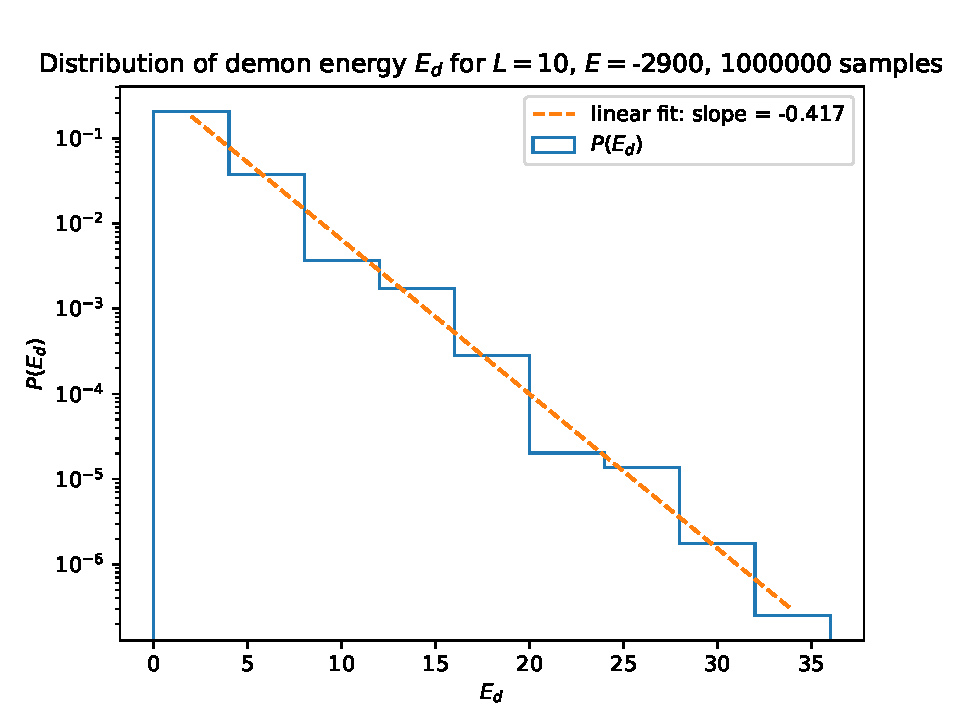
\includegraphics[width=0.9\textwidth]{E_d_L10_E2900.pdf}
% 	\end{subfigure}%
% 	\begin{subfigure}{.5\textwidth}
% 		\centering
% 		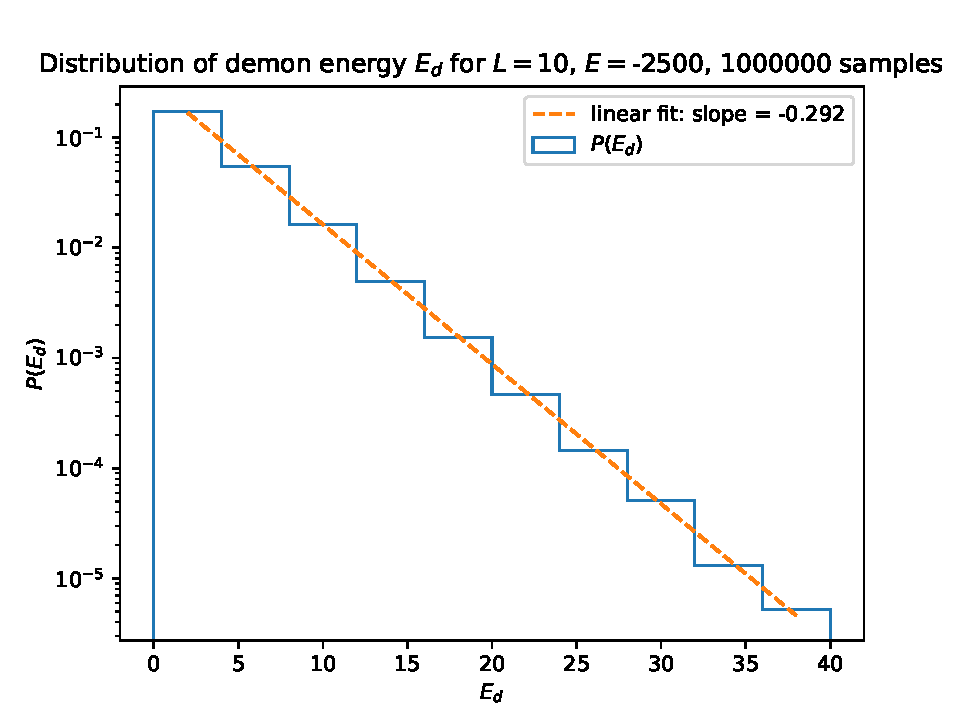
\includegraphics[width=0.9\textwidth]{E_d_L10_E2500.pdf}
% 	\end{subfigure}
% 	\begin{subfigure}{.5\textwidth}
% 		\centering
% 		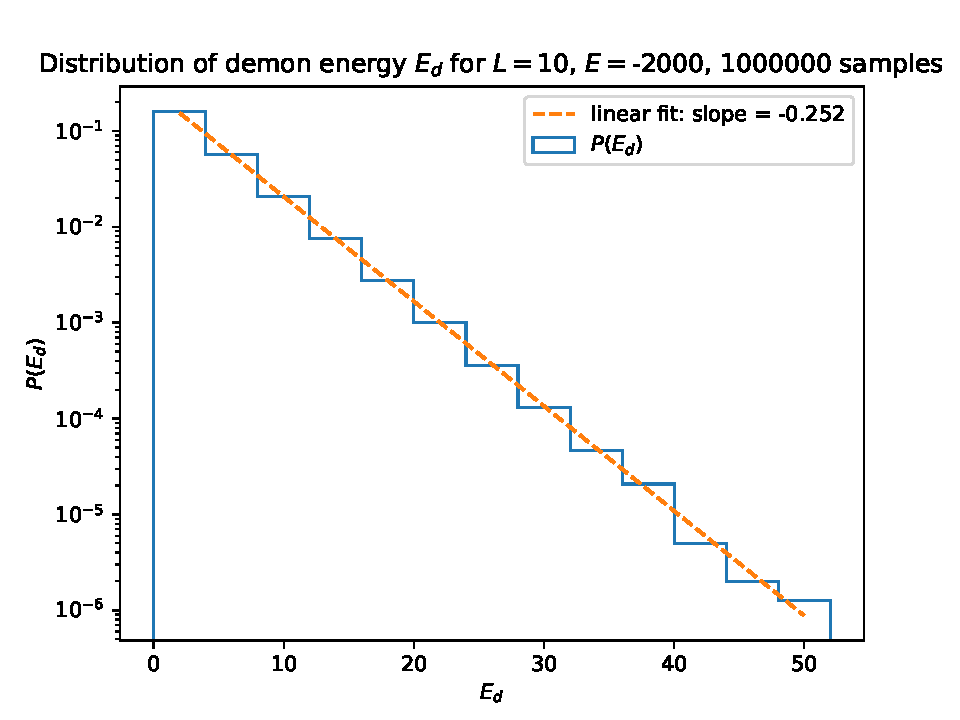
\includegraphics[width=0.9\textwidth]{E_d_L10_E2000.pdf}
% 	\end{subfigure}%
% 	\begin{subfigure}{.5\textwidth}
% 		\centering
% 		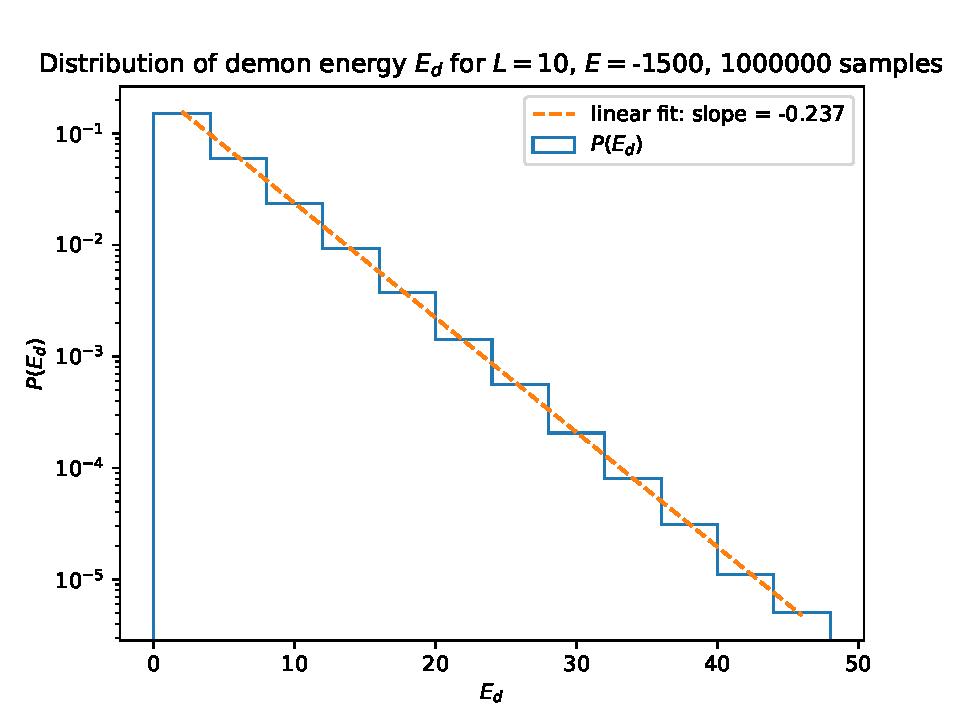
\includegraphics[width=0.9\textwidth]{E_d_L10_E1500.pdf}
% 	\end{subfigure}
% 	\begin{subfigure}{.5\textwidth}
% 		\centering
% 		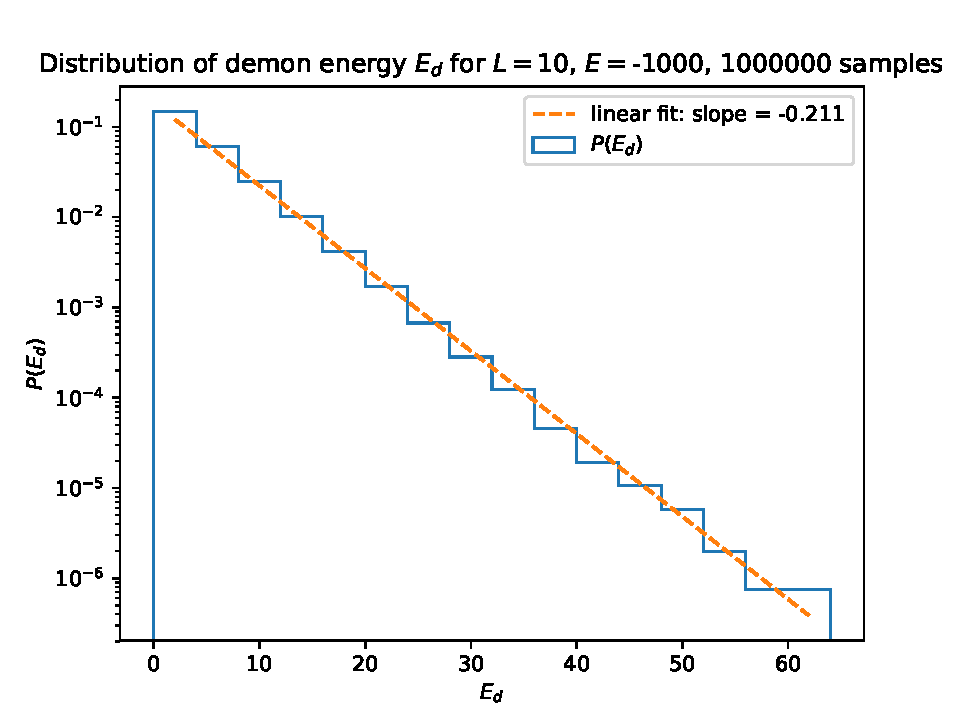
\includegraphics[width=0.9\textwidth]{E_d_L10_E1000.pdf}
% 	\end{subfigure}%
% 	\begin{subfigure}{.5\textwidth}
% 		\centering
% 		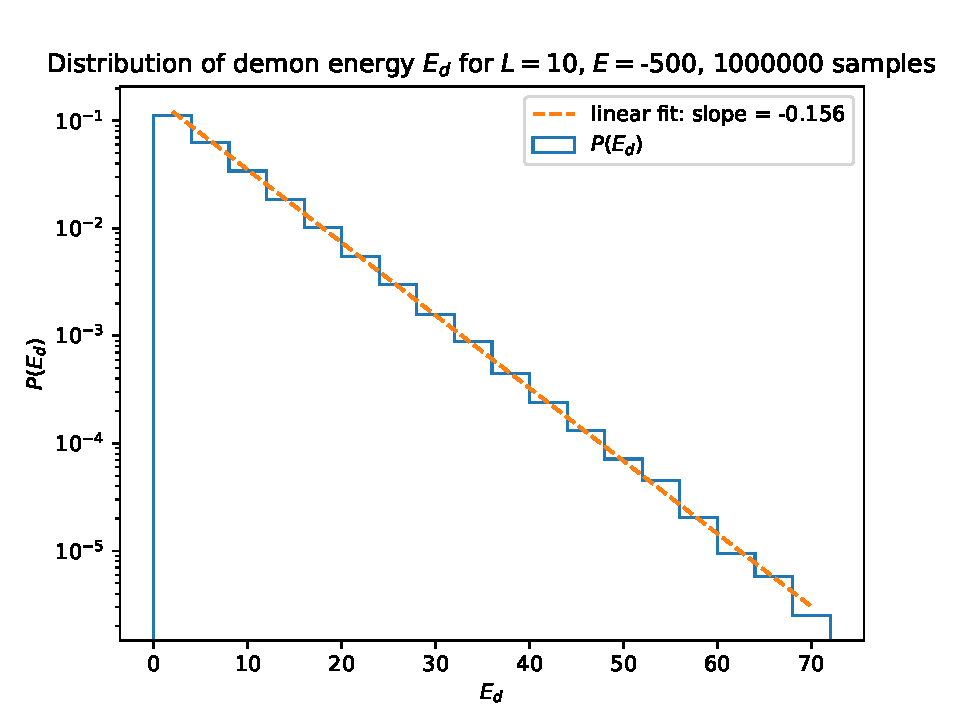
\includegraphics[width=0.9\textwidth]{E_d_L10_E500.pdf}
% 	\end{subfigure}
% 	\caption[short]{$P(E_d)$ plots for $L=10$}
% 	\label{fig:1}
% 	\end{figure}

\begin{figure}[b]
	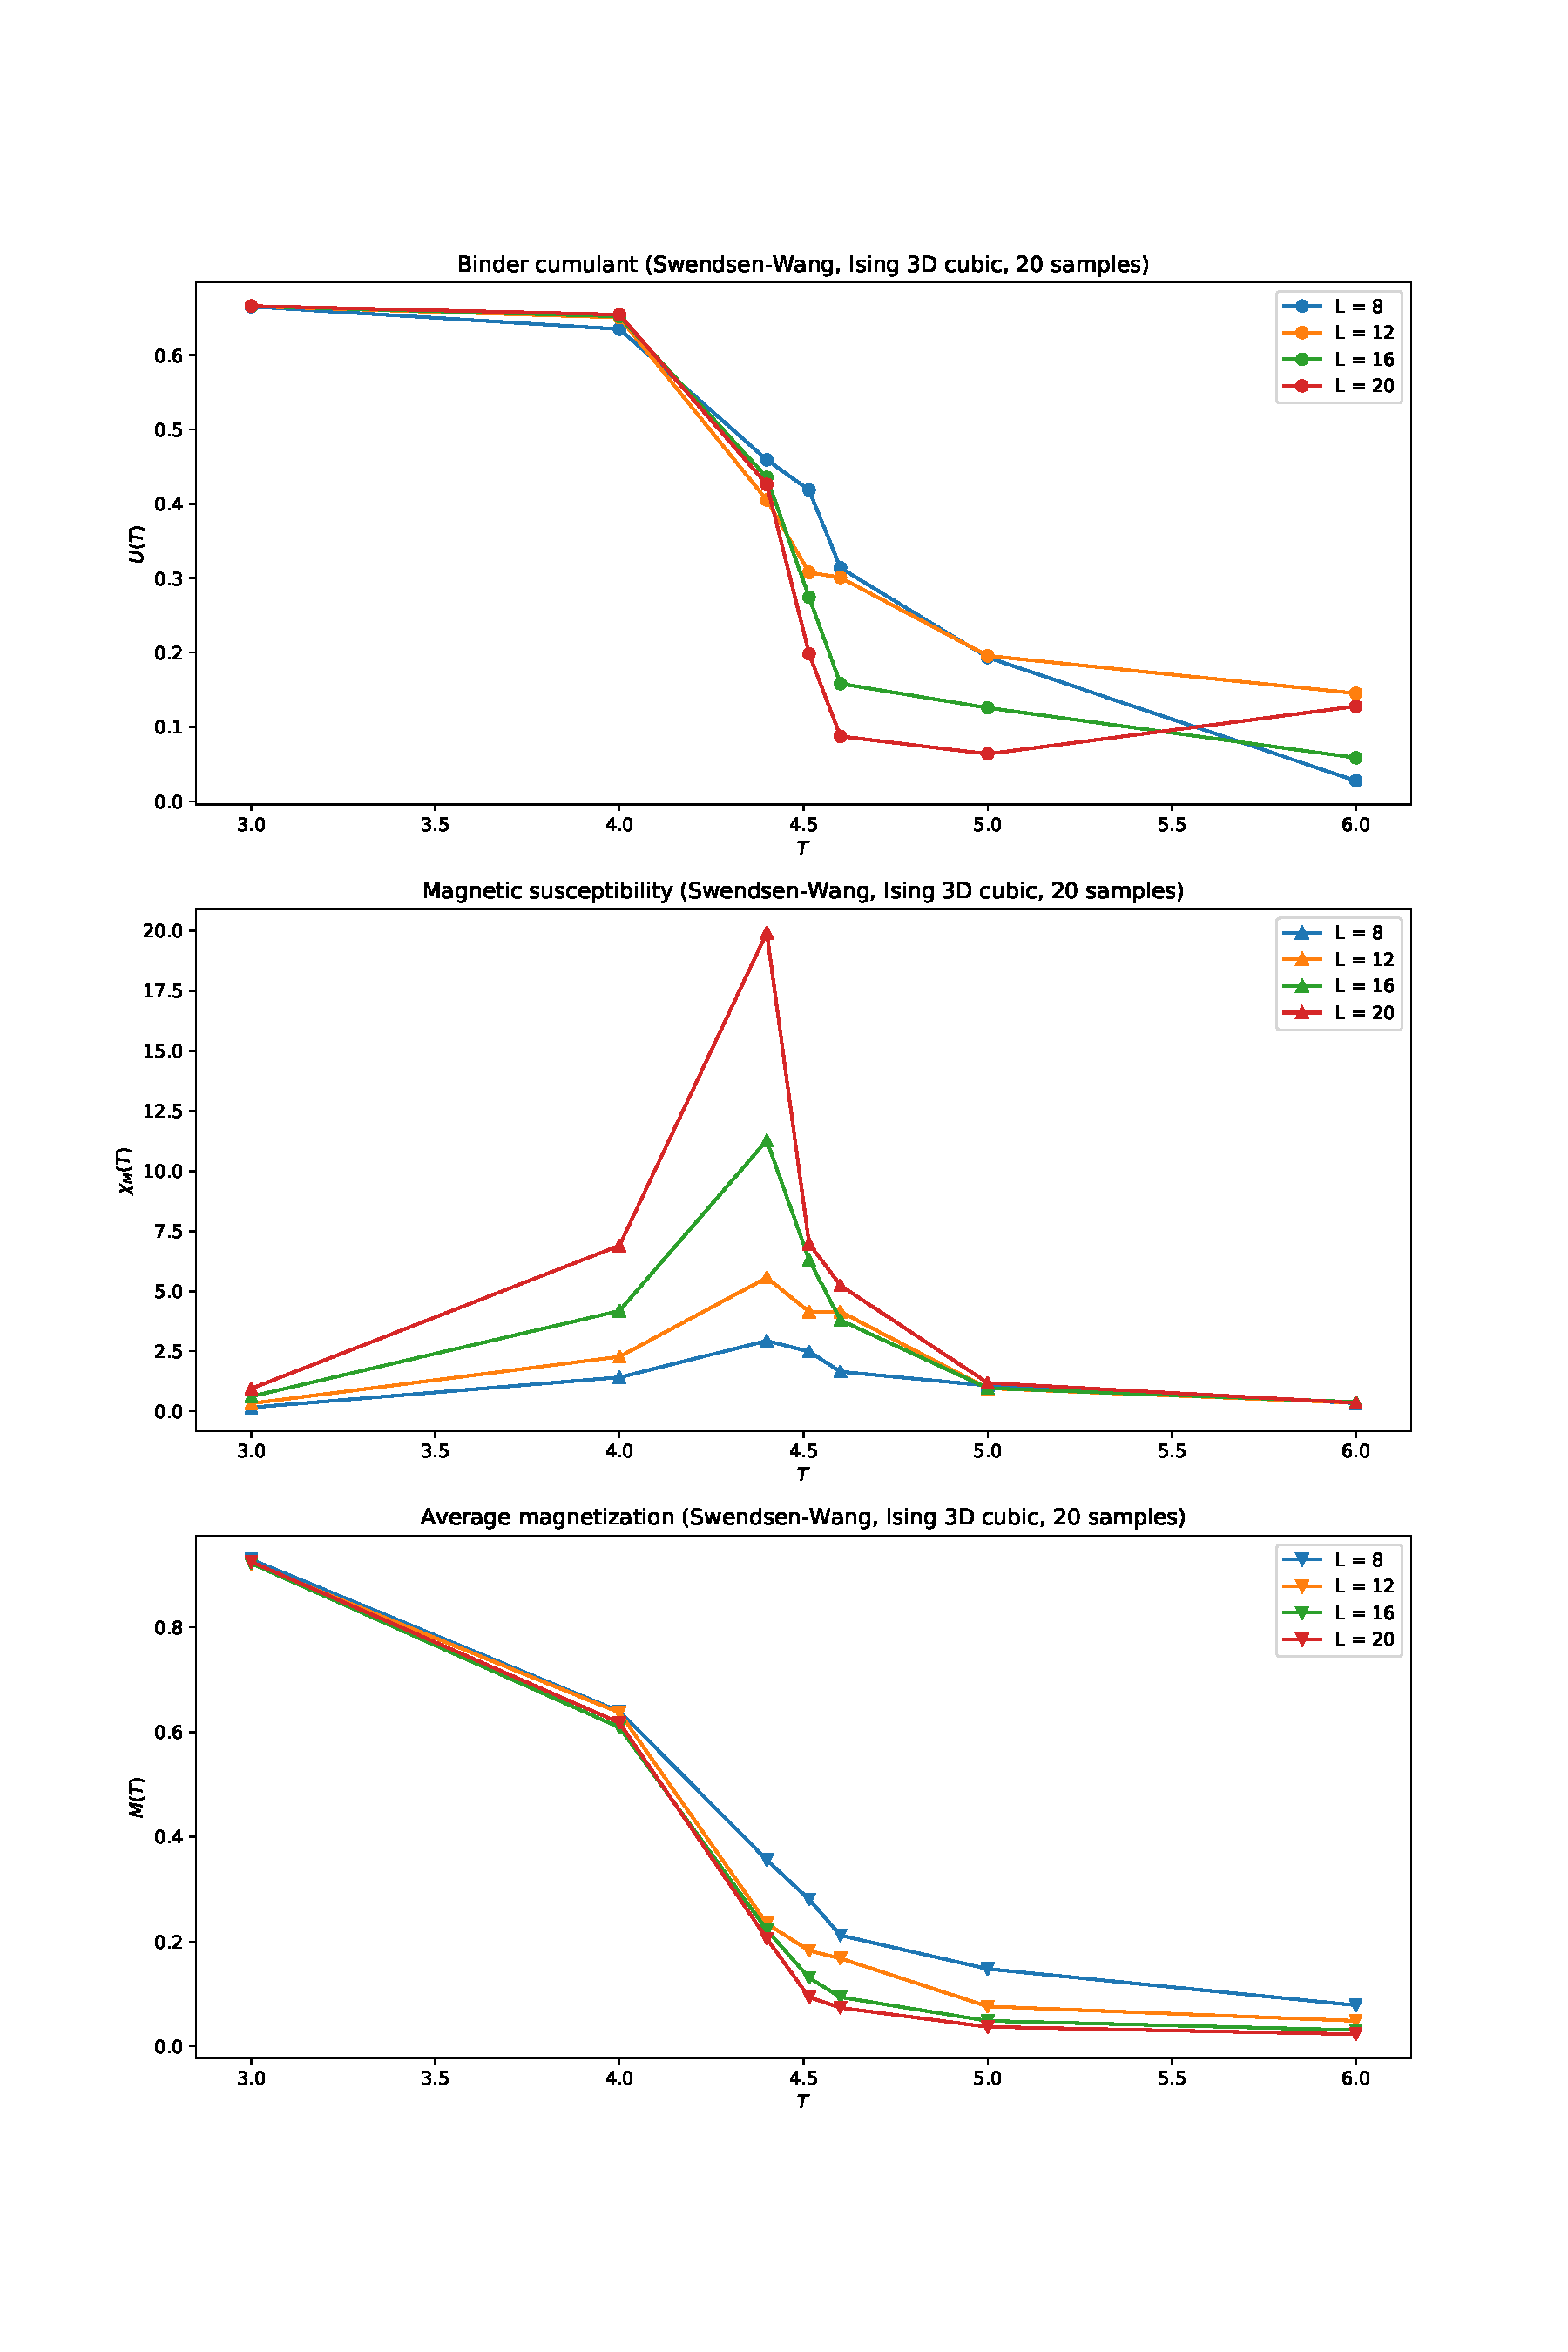
\includegraphics[width=0.9\textwidth]{Swendsen_Wang.pdf}
	\caption[short]{Results for Swendsen-Wang algorithm}
	\label{fig:1}
\end{figure}

\begin{figure}[b]
	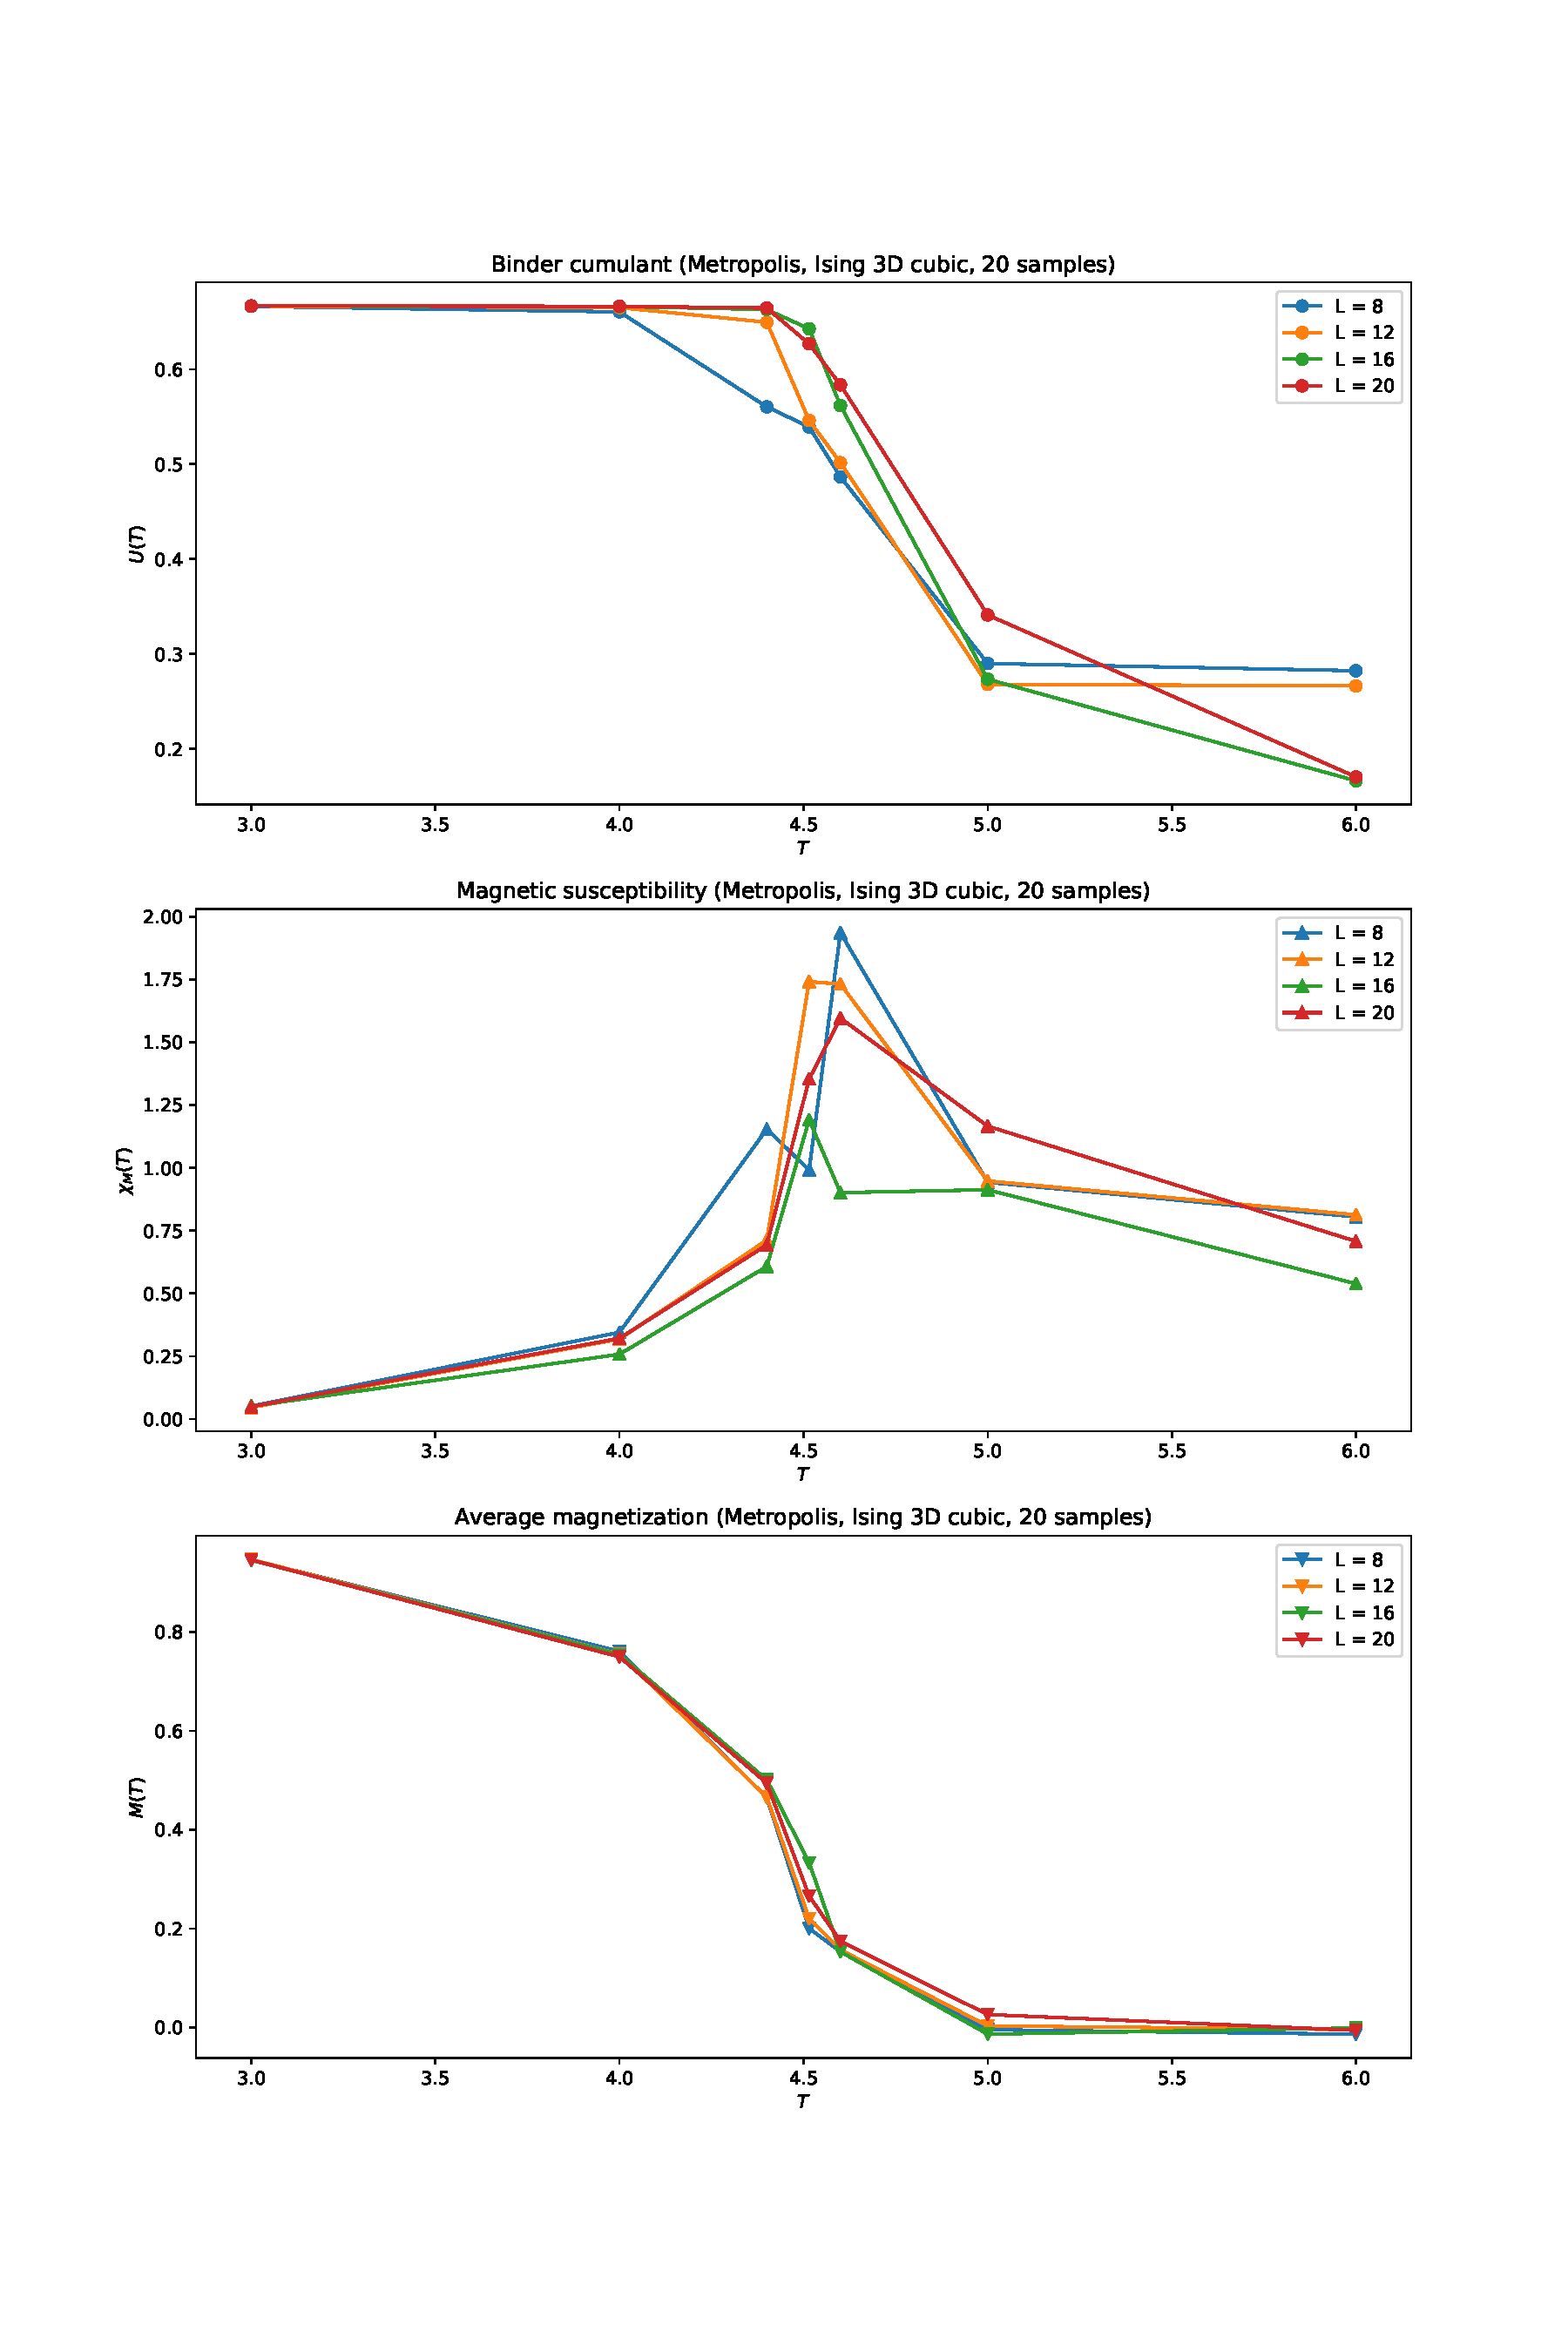
\includegraphics[width=0.9\textwidth]{Metropolis.pdf}
	\caption[short]{Results for Metropolis algorithm}
	\label{fig:2}
\end{figure}

Also, the autocorrelation $\rho_{MM}$ of magnetization $M$ was calculated once
thermalization was reached (figure~\ref{fig:3} and~\ref{fig:4}).

\begin{figure}[b]
	\centering
	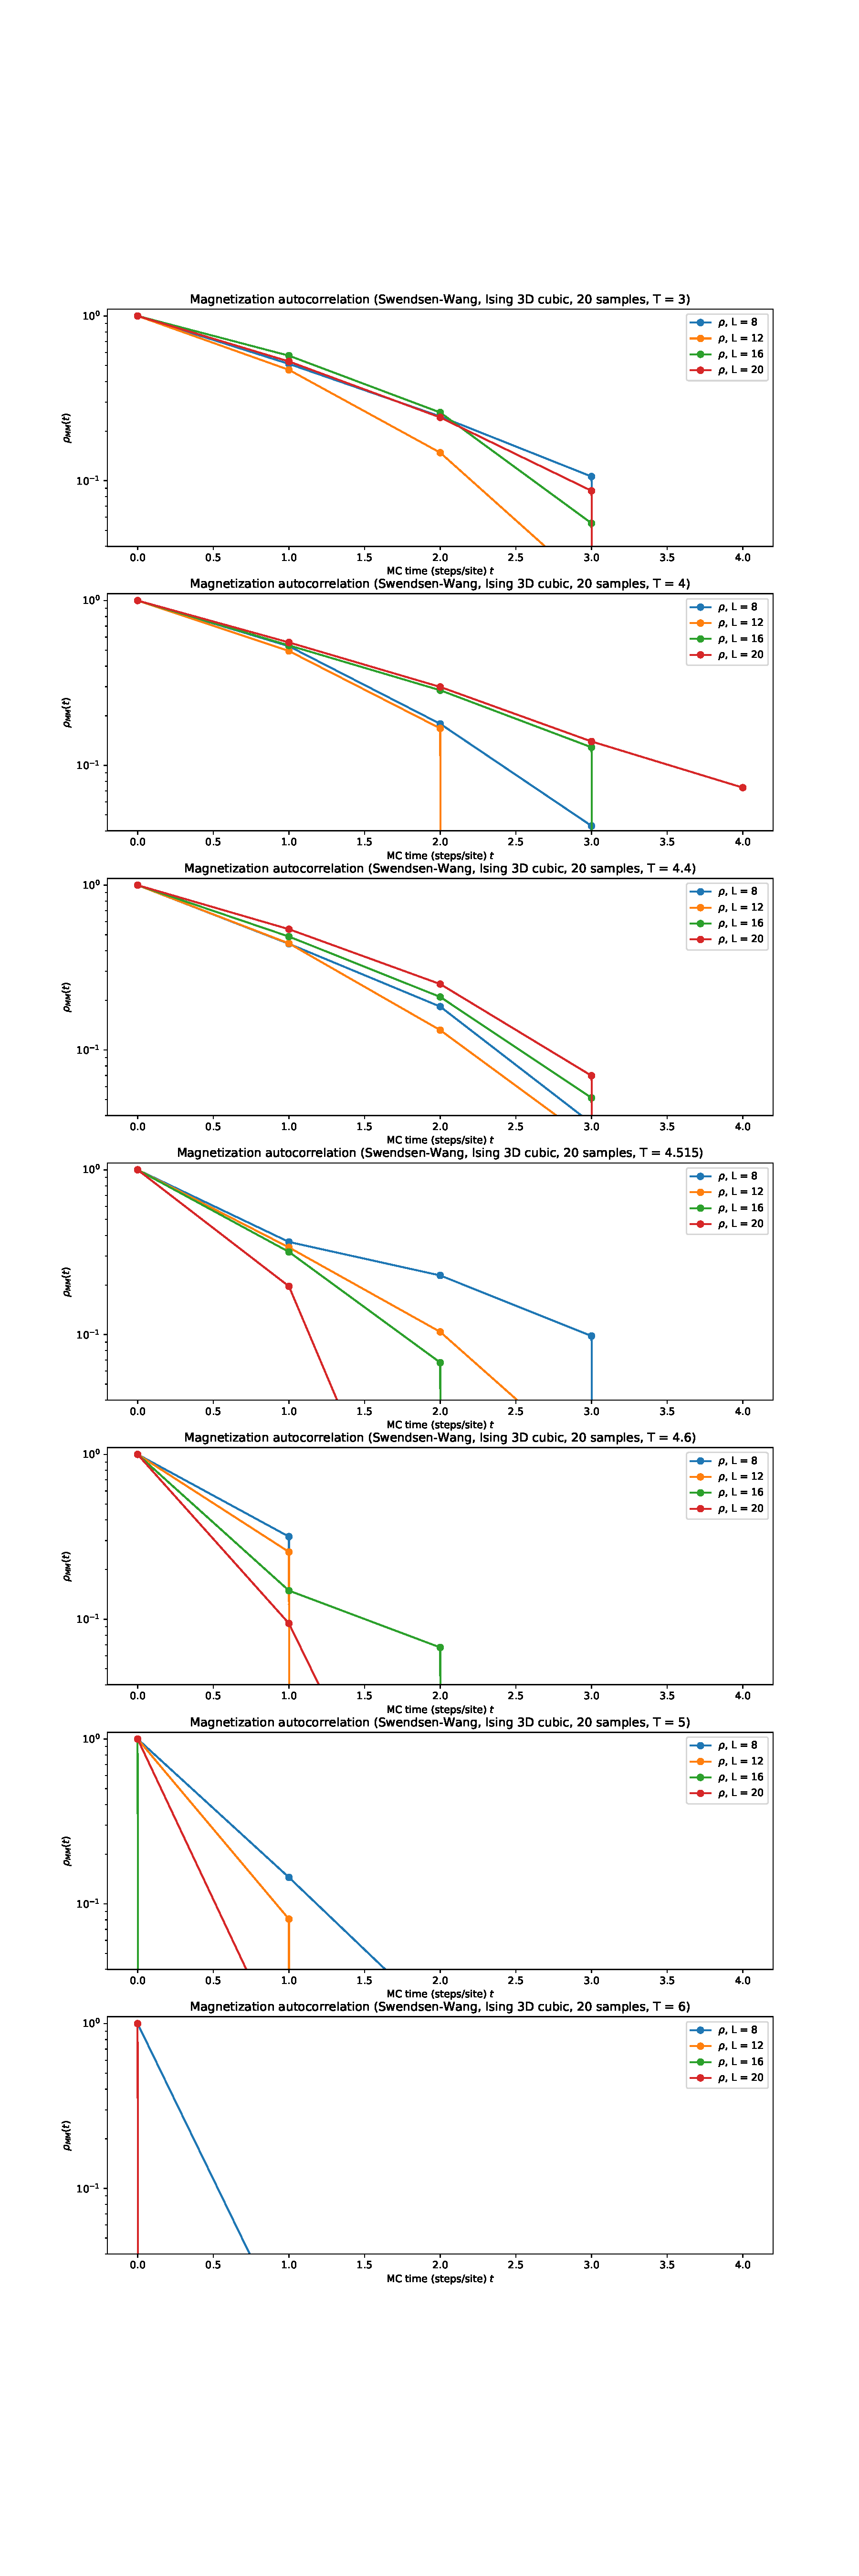
\includegraphics[height=26cm]{autocorr_Swendsen_Wang.pdf}
	\caption[short]{Autocorrelation behavior for Swendsen-Wang algorithm}
	\label{fig:3}
\end{figure}

\begin{figure}[b]
	\centering
	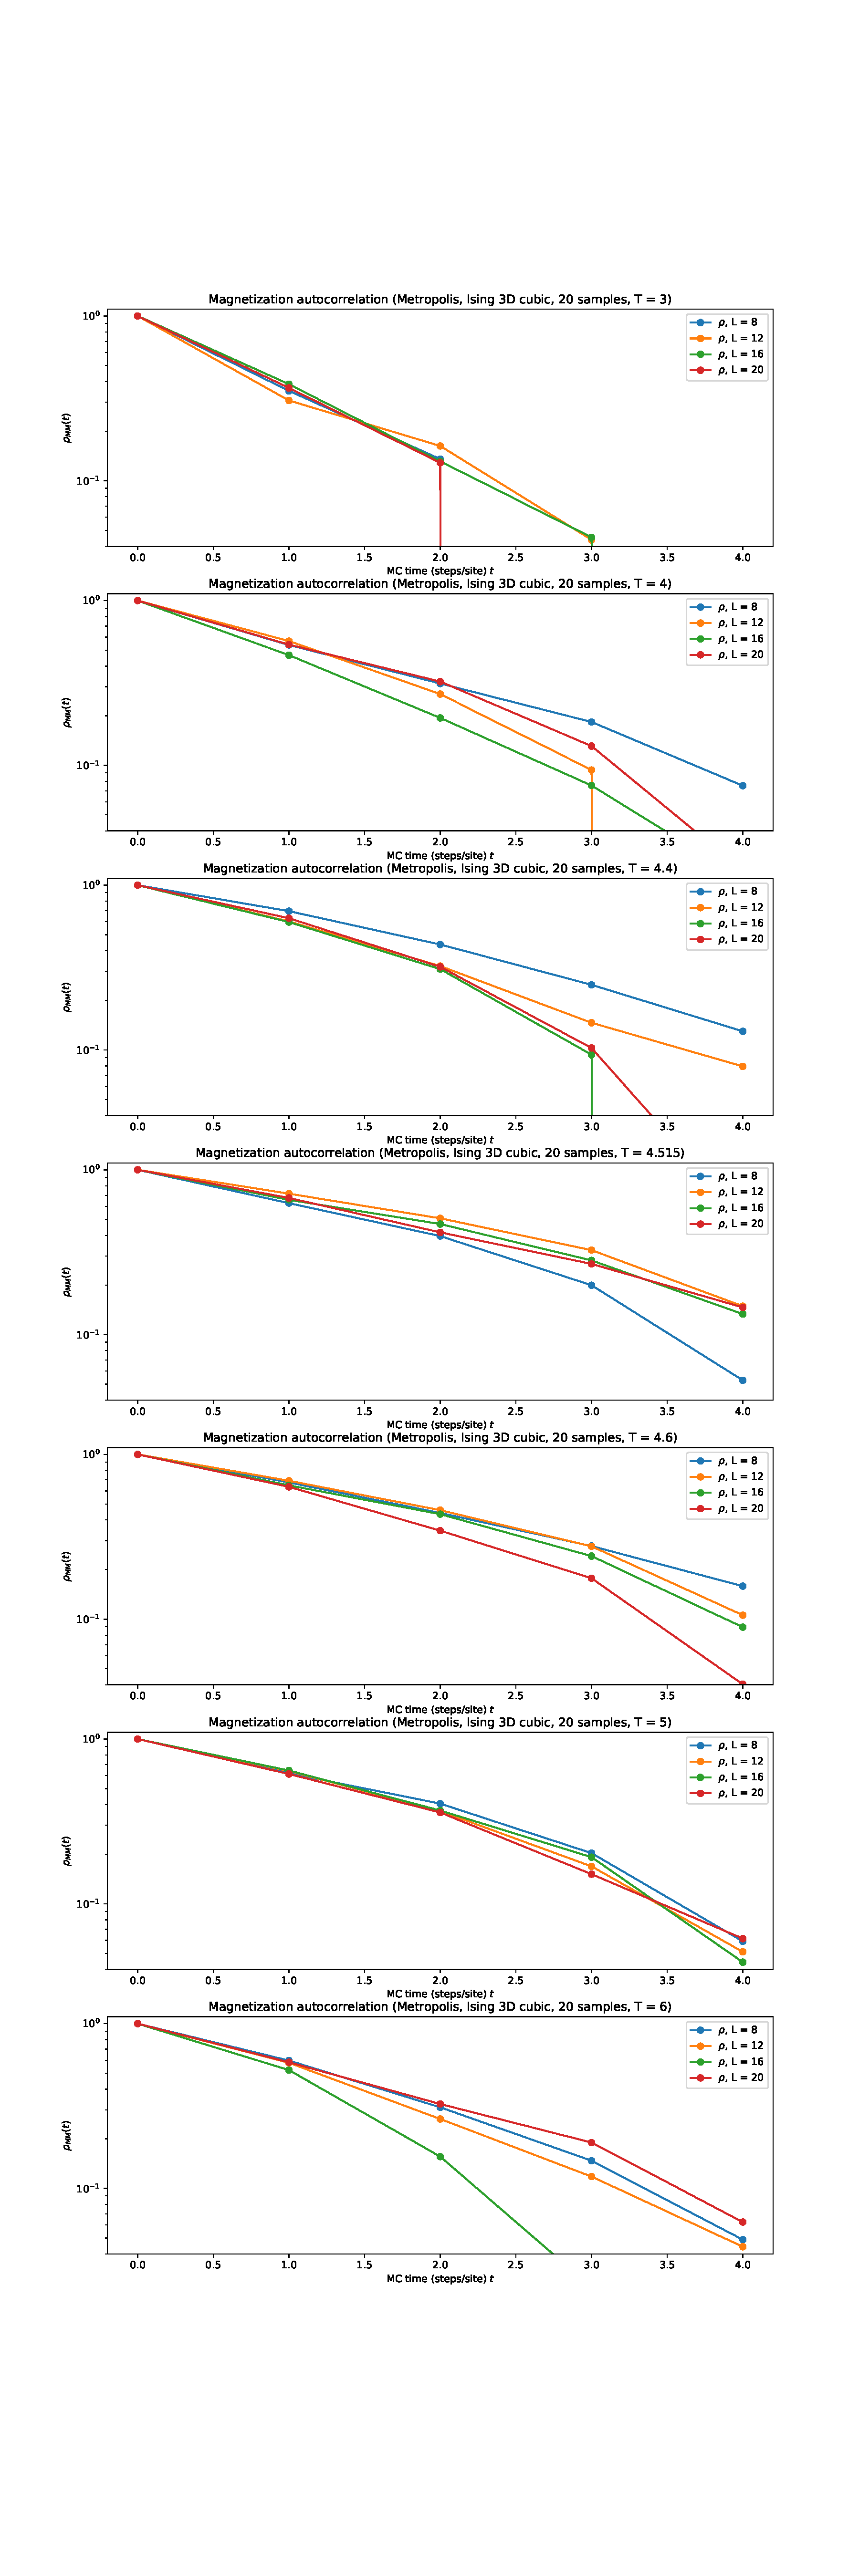
\includegraphics[height=26cm]{autocorr_Metropolis.pdf}
	\caption[short]{Autocorrelation behavior for Metropolis algorithm}
	\label{fig:4}
\end{figure}



Finally, autocorrelation time $\tau$ at critical temperature
$T_c \approx 4.515$ then was extracted from 
a semilog plot of $\rho_{MM}$ versus Monte Carlo time $t$ measured in steps per site using
the relationship $\rho_{MM} \sim e^{-t/\tau}$ (figure~\ref{fig:5} and~\ref{fig:6}).

\begin{figure}[b]
	\centering
	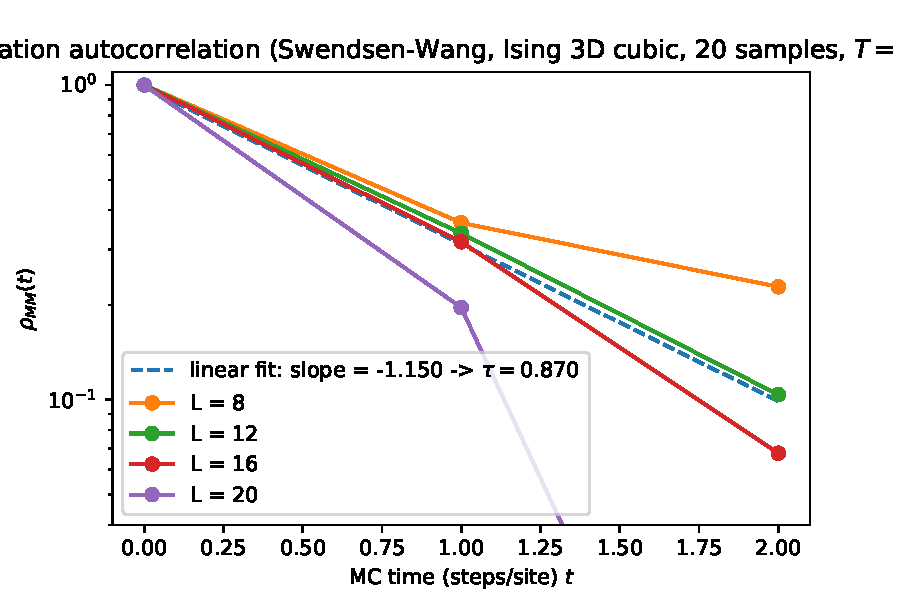
\includegraphics[width=0.7\textwidth]{tau_Swendsen_Wang.pdf}
	\caption[short]{Autocorrelation time for Swendsen-Wang algorithm}
	\label{fig:5}
\end{figure}

\begin{figure}[b]
	\centering
	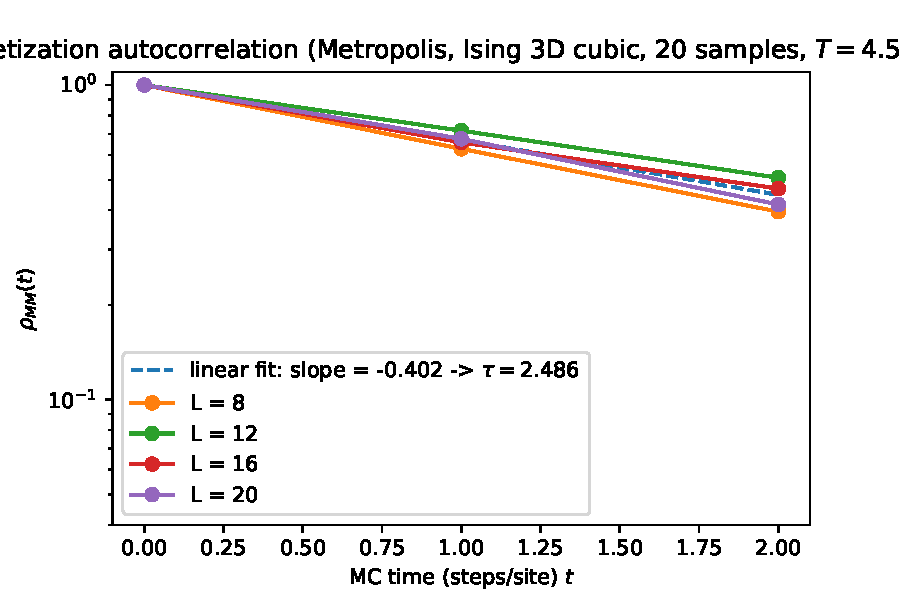
\includegraphics[width=0.7\textwidth]{tau_Metropolis.pdf}
	\caption[short]{Autocorrelation time for Metropolis algorithm}
	\label{fig:6}
\end{figure}


A comparison of actual simulation runtimes gives $0.141s$/sweep for the Swendsen-Wang algorithm
at $T=4.515$ and $L=20$ and $0.232s$/sweep for the Metropolis algorithm also at $T=4.515$ and $L=20$.
For this temperature and lattice size, we thus get $\text{MC}_{\text{speed:S-W}} = \frac{1\ \text{sweep}}{0.141 \text{s}}\frac{1}{0.87\ \text{sweep}}= \frac{8.152}{s}$
and $\text{MC}_{\text{speed:Metropolis}} = \frac{1\ \text{sweep}}{0.232 \text{s}}\frac{1}{2.486\ \text{sweep}}= \frac{1.731}{s}$.





\section{Discussion}
The plots of the magnetization, the magnetic susceptibility and the Binder cumulant 
seem as expected and in line with literature.
As expected, the autocorrelation behaviour shows critical slowing down for the Metropolis
algorithm around the critical temperature while the Swendsen-Wang algorithm remains largely unaffected.
The comparison of Monte Carlo speed shows that the Swendsen-Wang algorithm beats the metropolis
algorithm by a factor of 4.7 near critical temperature.\\
Qualitatively, all observations work out as expected from literature. However, the measured autocorrelation times
fall short of published values by a linear factor. In spite of spending a relevant amount of time looking for possible errors,
 I could not establish the reason.



\pagebreak
\begin{thebibliography}{99}

% \bibitem{creutz}
% 	Creutz, M.\\
% 	\emph{Microcanonical Monte Carlo Simulation},\\
% 	Phys. Rev. Lett. American Physical Society. 50 (19): 1411–1414,\\
% 	1983.

% \bibitem{herrmann}
% 	Herrmann, H. J.,
% 	Singer, H. M.,
% 	Mueller L.,
% 	Buchmann, M.-A.,\\
% 	\emph{Introduction to Computational Physics - Lecture Notes},\\
% 	ETH Zurich,\\
% 	2017.

\bibitem{metropolis}
	Metropolis, N.;
	Rosenbluth, A.W.;
	Rosenbluth, M.N.;
	Teller, A.H.;
	Teller, E.\\
	\emph{Equations of State Calculations by Fast Computing Machines},\\
	Journal of Chemical Physics. 21 (6): 1087\\
	1953.

\bibitem{swendsen}
	Swendsen, R. H.; Wang, J.-S.\\
	\emph{Nonuniversal critical dynamics in Monte Carlo simulations}\\
	Phys. Rev. Lett., 58(2):86–88\\
	1987

\bibitem{boettcher}
	Boettcher, L.,\\
	\emph{Computational Statistical Physics - Lecture Notes},\\
	ETH Zurich,\\
	2019.

\bibitem{galler}
	Galler, B. A.; Fischer, M. J.\\
	\emph{An improved equivalence algorithm},\\
	Communications of the ACM. 7.: 301–303,\\
	1964

\end{thebibliography}

\end{document}